%    Copyright © 2015
%  Eduardo Candido Xavier <eduardo@ic.unicamp.br>
%
%  This work is free. You can redistribute it and/or modify it under the
%  terms of the Do What The Fuck You Want To Public License, Version 2,
%  as published by Sam Hocevar. See the COPYING file for more details.
%
%  DO WHAT THE FUCK YOU WANT TO PUBLIC LICENSE
%                   Version 2, December 2004
%
%   Copyright (C) 2004 Sam Hocevar <sam@hocevar.net>
%
%   Everyone is permitted to copy and distribute verbatim or modified
%   copies of this license document, and changing it is allowed as long
%   as the name is changed.
%
%  DO WHAT THE FUCK YOU WANT TO PUBLIC LICENSE
%   TERMS AND CONDITIONS FOR COPYING, DISTRIBUTION AND MODIFICATION
%
%      0. You just DO WHAT THE FUCK YOU WANT TO.

\documentclass[handout]{beamer}
\usetheme{metropolis}
\beamertemplatetransparentcoveredhigh

\usepackage[portuges]{babel}
\usepackage{graphicx}
\graphicspath{{./figs/}}
\usepackage{listings}
\usepackage{color}
\usepackage{hyperref}
\usepackage{xpatch}
\usepackage[outputdir=build]{minted}

\makeatletter
\AtBeginEnvironment{minted}{\dontdofcolorbox}
\def\dontdofcolorbox{\renewcommand\fcolorbox[4][]{##4}}
\xpatchcmd{\inputminted}{\minted@fvset}{\minted@fvset\dontdofcolorbox}{}{}
\xpatchcmd{\mintinline}{\minted@fvset}{\minted@fvset\dontdofcolorbox}{}{}
\makeatother
\setminted[c]{
  linenos=true,
  breaklines=true,
  encoding=utf8,
  frame=lines,
  framerule=0.5pt,
  autogobble,
  fontsize=\small,
}
\setminted[bash]{
  linenos=true,
  encoding=utf8,
  frame=lines,
  framerule=0.5pt,
  autogobble,
  fontsize=\small
}

\newcommand{\cod}[1]{\mintinline{c}{#1}}


\definecolor{dkgreen}{rgb}{0,0.6,0}
\definecolor{gray}{rgb}{0.5,0.5,0.5}
\definecolor{mauve}{rgb}{0.58,0,0.82}


\definecolor{Purple}{HTML}{911146}
\definecolor{Orange}{HTML}{CF4A30}
\setbeamercolor{alerted text}{fg=Orange}
\setbeamercolor{frametitle}{bg=Purple}
\setbeamercolor{block body}{bg=Purple!20,fg=black}
\setbeamercolor{block title}{bg=Purple!50,fg=black}
\setbeamertemplate{blocks}[rounded][shadow=true]


\newcommand{\setcoverbg}{
  \setbeamertemplate{background}
  {
\includegraphics[width=\paperwidth,height=\paperheight]{backgrounds/coverbg}}
}
\newcommand{\setsectionbg}{
  \setbeamertemplate{background}
  {
\includegraphics[width=\paperwidth,height=\paperheight]{backgrounds/blank}}
}

\title{Programação Estruturada}
\subtitle{Estruturas de repetição}

\author{Professores Emílio Francesquini e Carla Negri Lintzmayer}
\institute{Centro de Matemática, Computação e Cognição\\ Universidade Federal do ABC}
\date{2018.Q3}

\begin{document}

\setcoverbg
\maketitle
\setsectionbg

%%%%%%%%%%%%%%%%%%%%%%%%%%%%%%%%%%%%%%%%%%%%%%%%%
%%%%%%%%%%%%%%%%%%%%%%%%%%%%%%%%%%%%%%%%%%%%%%%%%
%%%%%%%%%%%%%%%%%%%%%%%%%%%%%%%%%%%%%%%%%%%%%%%%%
%%%%%%%%%%%%%%%%%%%%%%%%%%%%%%%%%%%%%%%%%%%%%%%%%
%%%%%%%%%%%%%%%%%%%%%%%%%%%%%%%%%%%%%%%%%%%%%%%%%
%%%%%%%%%%%%%%%%%%%%%%%%%%%%%%%%%%%%%%%%%%%%%%%%%

\section{Comandos de repetição}%{{{

%%%%%%%%%%%%%%%%%%%%%%%%%%%%%%%%%%%%%%%%%%%%%%%%%
\begin{frame}{Comandos de repetição}
    \begin{itemize}[<+->]
        \item Até agora vimos como escrever programas capazes de executar comandos de forma linear, e, se necessário, tomar decisões com relação a executar ou não um bloco de comandos.
        \item Entretanto, eventualmente é necessário executar um bloco de comandos várias vezes para se obter o resultado esperado.
    \end{itemize}
\end{frame}

%%%%%%%%%%%%%%%%%%%%%%%%%%%%%%%%%%%%%%%%%%%%%%%%%
\begin{frame}[fragile]{Repetição}

    Vamos imprimir todos os números de 1 até 4.

    \begin{minted}{c}
        printf("1\n");
        printf("2\n");
        printf("3\n");
        printf("4\n");
    \end{minted}

    Dá para fazer com o que já vimos.
\end{frame}

%%%%%%%%%%%%%%%%%%%%%%%%%%%%%%%%%%%%%%%%%%%%%%%%%
\begin{frame}[fragile]{Repetição}

    Vamos imprimir todos os números de 1 até 100.

    \begin{minted}{c}
        printf("1\n");
        printf("2\n");
        printf("3\n");
        printf("4\n");
        printf("5\n");
        ...
        printf("100\n");
    \end{minted}

    Ainda dá para fazer com o que já vimos, mas é mais chato.
\end{frame}

%%%%%%%%%%%%%%%%%%%%%%%%%%%%%%%%%%%%%%%%%%%%%%%%%
\begin{frame}[fragile]{Repetição}

    Vamos imprimir todos os números de 1 até $n$, onde $n$ é informado pelo usuário.

    \begin{minted}[fontsize=\footnotesize]{c}
        scanf("%d", &n);
        if (n >= 1)
            printf("1\n");
        if (n >= 2)
            printf("2\n");
        if (n >= 3)
            printf("3\n");
        ...
        if (n >= 100)
            printf("100\n");
    \end{minted}

    \pause
    Agora ficou impossível!

    Note que esse programa é válido apenas para $n \leq 100$.
\end{frame}

%}}}
%%%%%%%%%%%%%%%%%%%%%%%%%%%%%%%%%%%%%%%%%%%%%%%%%
%%%%%%%%%%%%%%%%%%%%%%%%%%%%%%%%%%%%%%%%%%%%%%%%%
%%%%%%%%%%%%%%%%%%%%%%%%%%%%%%%%%%%%%%%%%%%%%%%%%
%%%%%%%%%%%%%%%%%%%%%%%%%%%%%%%%%%%%%%%%%%%%%%%%%
%%%%%%%%%%%%%%%%%%%%%%%%%%%%%%%%%%%%%%%%%%%%%%%%%
%%%%%%%%%%%%%%%%%%%%%%%%%%%%%%%%%%%%%%%%%%%%%%%%%

\section{Comando {\bf while}}%{{{

%%%%%%%%%%%%%%%%%%%%%%%%%%%%%%%%%%%%%%%%%%%%%%%%%
\begin{frame}[fragile]{Comando {\bf while}}

    Estrutura:

    \begin{minted}{c}
        while (condição)
            comando;
    \end{minted}

    ou

    \begin{minted}{c}
        while (condição) {
            comandos;
        }
    \end{minted}

    Enquanto a condição for verdadeira ($\neq 0$), o(s) comando(s) são executados.
\end{frame}

%%%%%%%%%%%%%%%%%%%%%%%%%%%%%%%%%%%%%%%%%%%%%%%%%
\begin{frame}[fragile]{Comando {\bf while}}

    \begin{description}
        \item[Passo 1] Testa a condição. Se ela for verdadeira, vai para o Passo 2. Se for falsa, vai para o Passo 3.
        \item[Passo 2] Executa os comandos. Vai para o Passo 1.
        \item[Passo 3] Segue o programa.
    \end{description}

    \begin{center}
        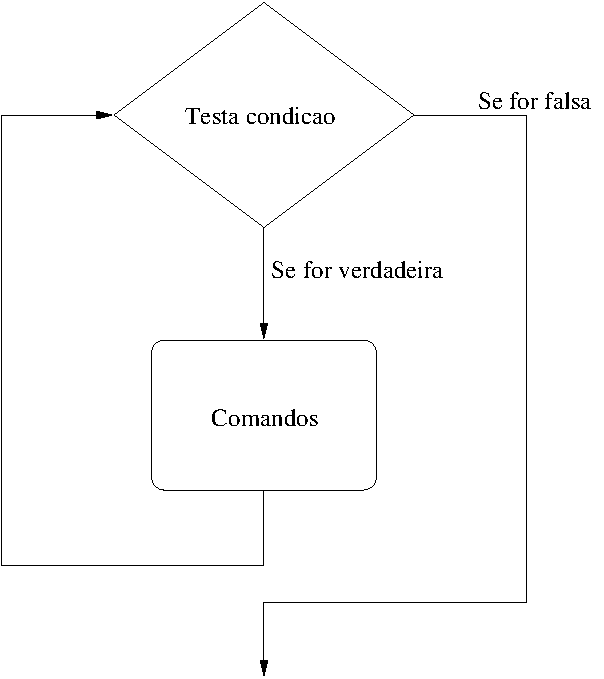
\includegraphics[width=0.45\textwidth]{figs/while}
    \end{center}
\end{frame}

%%%%%%%%%%%%%%%%%%%%%%%%%%%%%%%%%%%%%%%%%%%%%%%%%
\begin{frame}[fragile]{Comando {\bf while}}

    Vamos imprimir todos os números de 1 até 100.

    \begin{minted}{c}
        #include <stdio.h>

        int main() {
            int i;

            i = 1;
            while (i <= 100) {
                printf("%d\n", i);
                i++;
            }

            return 0;
        }
    \end{minted}
\end{frame}

%%%%%%%%%%%%%%%%%%%%%%%%%%%%%%%%%%%%%%%%%%%%%%%%%
\begin{frame}[fragile]{Comando {\bf while}}

    Vamos imprimir todos os números de 1 até $n$.

    \begin{minted}{c}
        #include <stdio.h>

        int main() {
            int i, n;

            scanf("%d", &n);
            i = 1;
            while (i <= n) {
                printf("%d\n", i);
                i++;
            }

            return 0;
        }
    \end{minted}
\end{frame}

%%%%%%%%%%%%%%%%%%%%%%%%%%%%%%%%%%%%%%%%%%%%%%%%%
\begin{frame}[fragile]{Comando {\bf while}}

    \begin{itemize}[<+->]
        \item O que acontece se a condição for falsa na primeira vez?
        \begin{minted}{c}
            while (a != a)
                a = a + 1;
        \end{minted}
        %{\bf Resposta:} Ele nunca entra na repetição (no laço).

        \item O que acontece se a condição for sempre verdadeira?
        \begin{minted}{c}
            while (a == a)
                a = a + 1;
        \end{minted}
        %{\bf Resposta:} Ele entra na repetição e nunca sai (laço infinito).
    \end{itemize}
\end{frame}
%}}}
%%%%%%%%%%%%%%%%%%%%%%%%%%%%%%%%%%%%%%%%%%%%%%%%%
%%%%%%%%%%%%%%%%%%%%%%%%%%%%%%%%%%%%%%%%%%%%%%%%%
%%%%%%%%%%%%%%%%%%%%%%%%%%%%%%%%%%%%%%%%%%%%%%%%%
%%%%%%%%%%%%%%%%%%%%%%%%%%%%%%%%%%%%%%%%%%%%%%%%%
%%%%%%%%%%%%%%%%%%%%%%%%%%%%%%%%%%%%%%%%%%%%%%%%%
%%%%%%%%%%%%%%%%%%%%%%%%%%%%%%%%%%%%%%%%%%%%%%%%%

\section{Comando {\bf do-while}}%{{{
%%%%%%%%%%%%%%%%%%%%%%%%%%%%%%%%%%%%%%%%%%%%%%%%%

\begin{frame}[fragile]{Comando {\bf do-while}}

    Estrutura:
    \begin{minted}{c}
        do
            comando;
        while (condição);
    \end{minted}

    ou

    \begin{minted}{c}
        do {
            comandos;
        } while (condição);
    \end{minted}

    \pause
    Diferença do {\bf while}: sempre executa o(s) comando(s) pelo menos uma vez.

    O teste condicional é feito por último.
\end{frame}

%%%%%%%%%%%%%%%%%%%%%%%%%%%%%%%%%%%%%%%%%%%%%%%%%
\begin{frame}[fragile]{Comando {\bf do-while}}

    \begin{description}
        \item[Passo 1] Executa os comandos. Vai para o Passo 2.
        \item[Passo 2] Testa a condição. Se ela for verdadeira, vai para Passo 1. Se for falsa, vai para o Passo 3.
        \item[Passo 3] Segue o programa.
    \end{description}

    \begin{center}
        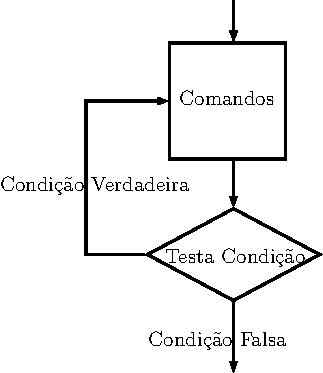
\includegraphics[width=0.4\textwidth]{figs/do-while}
    \end{center}
\end{frame}

%%%%%%%%%%%%%%%%%%%%%%%%%%%%%%%%%%%%%%%%%%%%%%%%%
\begin{frame}[fragile]{Comando {\bf do-while}}

    Vamos imprimir todos os números de 1 até 100.

    \begin{minted}{c}
        #include <stdio.h>

        int main() {
            int i;

            i = 1;
            do {
                printf("%d\n", i);
                i = i + 1;
            } while (i <= 100);

            return 0;
        }
    \end{minted}
\end{frame}

%%%%%%%%%%%%%%%%%%%%%%%%%%%%%%%%%%%%%%%%%%%%%%%%%
\begin{frame}[fragile]{Comando {\bf do-while}}

    Vamos imprimir todos os números de 1 até $n$.

    \begin{minted}[fontsize=\scriptsize]{c}
        #include <stdio.h>

        int main() {
            int i, n;

            scanf("%d", &n);
            i = 1;
            do {
                printf("%d\n", i);
                i = i + 1;
            } while (i <= n);

            return 0;
        }
    \end{minted}

    \pause
    E se o usuário digitar 0?
\end{frame}
%}}}
%%%%%%%%%%%%%%%%%%%%%%%%%%%%%%%%%%%%%%%%%%%%%%%%%
%%%%%%%%%%%%%%%%%%%%%%%%%%%%%%%%%%%%%%%%%%%%%%%%%
%%%%%%%%%%%%%%%%%%%%%%%%%%%%%%%%%%%%%%%%%%%%%%%%%
%%%%%%%%%%%%%%%%%%%%%%%%%%%%%%%%%%%%%%%%%%%%%%%%%
%%%%%%%%%%%%%%%%%%%%%%%%%%%%%%%%%%%%%%%%%%%%%%%%%
%%%%%%%%%%%%%%%%%%%%%%%%%%%%%%%%%%%%%%%%%%%%%%%%%

\section{O comando {\bf for}}%{{{
%%%%%%%%%%%%%%%%%%%%%%%%%%%%%%%%%%%%%%%%%%%%%%%%%

\begin{frame}[fragile]{O comando {\bf for}}
    \small
    Estrutura:
    \begin{minted}[fontsize=\footnotesize]{c}
        for (início; condição; passo)
            comando;
    \end{minted}
    \vskip -0.5cm
    ou
    \begin{minted}[fontsize=\footnotesize]{c}
        for (início; condição; passo) {
            comandos;
        }
    \end{minted}

    \begin{itemize}
        \item {\bf Início}: uma ou mais atribuições, separadas por ``,''
        \item {\bf Condição}: os comandos são executados enquanto a condição for verdadeira
        \item {\bf Passo}: um ou mais comandos separados por ``,''. Os comandos do passo sempre são executados após os comandos do bloco
    \end{itemize}
\end{frame}

%%%%%%%%%%%%%%%%%%%%%%%%%%%%%%%%%%%%%%%%%%%%%%%%%
\begin{frame}[fragile]{O comando {\bf for}}

    \begin{minipage}{0.55\textwidth}
        \small
        \begin{description}
            \item[Passo 1] Executa os comandos em ``início''. Vai para Passo 2.
            \item[Passo 2] Testa a condição. Se ela for verdadeira, vai para Passo 3. Se for falsa, vai para Passo 5.
            \item[Passo 3] Executa os comandos do bloco. Vai para Passo 4.
            \item[Passo 4] Executa os comandos em ``passo''. Vai para Passo 2.
            \item[Passo 5] Segue o programa.
        \end{description}
    \end{minipage}
    \hfill
    \begin{minipage}{0.4\textwidth}
        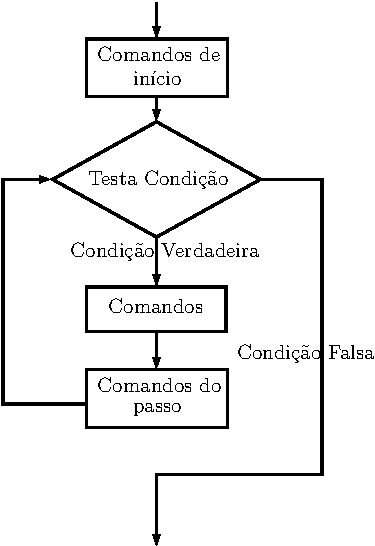
\includegraphics[width=\textwidth]{figs/for}
    \end{minipage}
\end{frame}

%%%%%%%%%%%%%%%%%%%%%%%%%%%%%%%%%%%%%%%%%%%%%%%%%
\begin{frame}[fragile]{O comando {\bf for}}

    O {\bf for} é equivalente à seguinte construção utilizando o {\bf while}:

    \begin{minted}{c}
        início;
        while (condição) {
            comandos;
            passo;
        }
    \end{minted}
\end{frame}

%%%%%%%%%%%%%%%%%%%%%%%%%%%%%%%%%%%%%%%%%%%%%%%%%
\begin{frame}[fragile]{O comando {\bf for}}

    Vamos imprimir todos os números de 1 até 100.

    \begin{minted}{c}
        #include <stdio.h>

        int main() {
            int i;

            for (i = 1; i <= 100; i++) {
                printf("%d\n", i);
            }

            return 0;
        }
    \end{minted}
\end{frame}

%%%%%%%%%%%%%%%%%%%%%%%%%%%%%%%%%%%%%%%%%%%%%%%%%
\begin{frame}[fragile]{O comando {\bf for}}

    Vamos imprimir todos os números de 1 até $n$.

    \begin{minted}{c}
        #include <stdio.h>

        int main() {
            int i, n;

            scanf("%d", &n);
            for (i = 1; i <= n; i++) {
                printf("%d\n", i);
            }

            return 0;
        }
    \end{minted}
\end{frame}

%%%%%%%%%%%%%%%%%%%%%%%%%%%%%%%%%%%%%%%%%%%%%%%%%
\begin{frame}{I'll not throw paper airplanes in class}
    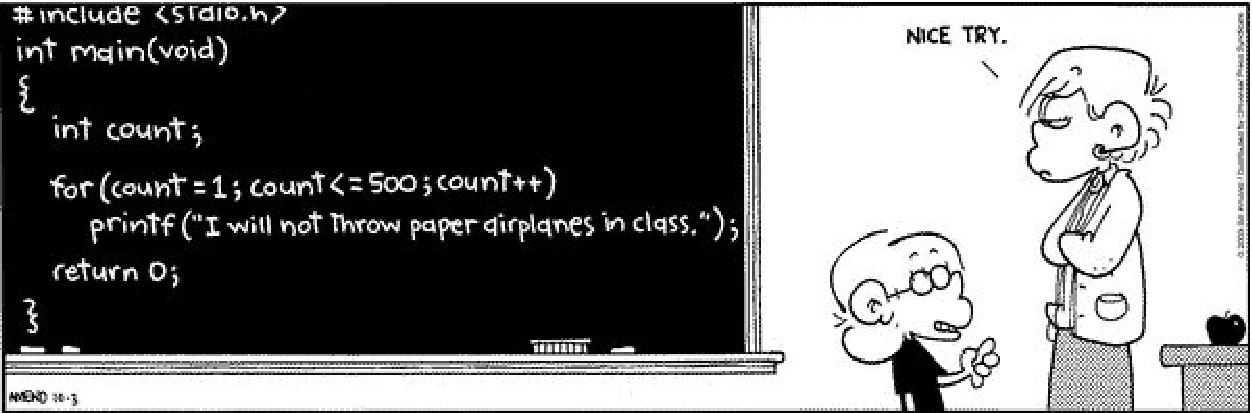
\includegraphics[width=\textwidth]{figs/joke}
\end{frame}
%}}}
%%%%%%%%%%%%%%%%%%%%%%%%%%%%%%%%%%%%%%%%%%%%%%%%%
%%%%%%%%%%%%%%%%%%%%%%%%%%%%%%%%%%%%%%%%%%%%%%%%%
%%%%%%%%%%%%%%%%%%%%%%%%%%%%%%%%%%%%%%%%%%%%%%%%%
%%%%%%%%%%%%%%%%%%%%%%%%%%%%%%%%%%%%%%%%%%%%%%%%%
%%%%%%%%%%%%%%%%%%%%%%%%%%%%%%%%%%%%%%%%%%%%%%%%%
%%%%%%%%%%%%%%%%%%%%%%%%%%%%%%%%%%%%%%%%%%%%%%%%%

\section{Comandos {\bf continue} e {\bf break}}%{{{

%%%%%%%%%%%%%%%%%%%%%%%%%%%%%%%%%%%%%%%%%%%%%%%%%
\begin{frame}[fragile]{Laços e o comando {\bf break}}

    O comando {\bf break} faz com que a execução de um laço seja terminada, passando a execução para o próximo comando depois do final do laço.

    \begin{minted}{c}
        int i;

        for (i = 1; i <= 10; i++) {
            if (i >= 5)
                break;
            printf("%d\n", i);
        }

        printf("Terminou o laço\n");
    \end{minted}

    O que será impresso?
    %{\bf Resposta:} Os números de 1 até 4 e depois a frase ``Terminou o laço".
\end{frame}

%%%%%%%%%%%%%%%%%%%%%%%%%%%%%%%%%%%%%%%%%%%%%%%%%
\begin{frame}[fragile]{Laços e o comando {\bf break}}

    Assim como a ``condição'' em laços, o comando {\bf break} é utilizado em situações de parada de um laço.

    Ex.: Imprimindo os números de 1 até 10.

    \begin{minted}[fontsize=\scriptsize]{c}
        int i;
        for (i = 1; ; i++) {
            if (i > 10)
                break;
            printf("%d\n", i);
        }
    \end{minted}

    é equivalente a:

    \begin{minted}[fontsize=\scriptsize]{c}
        int i;
        for (i = 1; i <= 10; i++) {
            printf("%d\n", i);
        }
    \end{minted}
\end{frame}

%%%%%%%%%%%%%%%%%%%%%%%%%%%%%%%%%%%%%%%%%%%%%%%%
\begin{frame}[fragile]{Laços e o comando {\bf continue}}

    O comando {\bf continue} faz com que a execução de um laço seja alterada para o final do laço.

    \begin{minted}{c}
        int i;
        for (i = 1; i <= 10; i++) {
            if (i == 5)
                continue;
            printf("%d\n", i);
        }
        printf("Terminou o laço\n");
    \end{minted}

    O que será impresso?
    %{\bf Resposta:} Os números de 1 até 10, exceto o número 5, e depois a frase ``Terminou o laço".
\end{frame}

%%%%%%%%%%%%%%%%%%%%%%%%%%%%%%%%%%%%%%%%%%%%%%%%
\begin{frame}[fragile]{Laços e o comando {\bf continue}}

    O {\bf continue} é utilizado em situações onde comandos dentro do laço só devem ser executados caso alguma condição seja satisfeita.

    Ex.: Imprimindo área de um círculo, mas apenas se o raio for par e estiver entre 1 e 10.

    \begin{minted}{c}
        int r;
        double area;
        for (r = 1; r <= 10; r++) {
            if ((r % 2) != 0) /* se número for ímpar pulamos */
                continue;
            area = 3.1415 * r * r;
            printf("%lf\n", area);
        }
    \end{minted}

    Mas note que poderíamos escrever algo mais simples:

    \begin{minted}{c}
        int r;
        double area;
        for (r = 2; r <= 10; r = r+2) {
            area = 3.1415 * r * r;
            printf("%lf\n", area);
        }
    \end{minted}
\end{frame}
%}}}
%%%%%%%%%%%%%%%%%%%%%%%%%%%%%%%%%%%%%%%%%%%%%%%
%%%%%%%%%%%%%%%%%%%%%%%%%%%%%%%%%%%%%%%%%%%%%%%
%%%%%%%%%%%%%%%%%%%%%%%%%%%%%%%%%%%%%%%%%%%%%%%
%%%%%%%%%%%%%%%%%%%%%%%%%%%%%%%%%%%%%%%%%%%%%%%
%%%%%%%%%%%%%%%%%%%%%%%%%%%%%%%%%%%%%%%%%%%%%%%
%%%%%%%%%%%%%%%%%%%%%%%%%%%%%%%%%%%%%%%%%%%%%%%

\section{Laços encaixados}%{{{

%%%%%%%%%%%%%%%%%%%%%%%%%%%%%%%%%%%%%%%%%%%%%%%
\begin{frame}[fragile]{Laços encaixados}
    
    \begin{itemize}
        \item Para resolver alguns problemas, é necessário implementar um laço dentro de outro laço.
        \item Estes são conhecidos como laços encaixados (ou aninhados).
        
        \begin{minted}{c}
            int main() {
                int i, j;
                
                for (i = 1; i <= 4; i++)
                    for (j = 1; j <= 3; j++)
                        printf("%d %d\n", i, j);

                return 0;
            }
        \end{minted}
    
        \item O que será impresso por este programa?
    \end{itemize}
\end{frame}

%%%%%%%%%%%%%%%%%%%%%%%%%%%%%%%%%%%%%%%%%%%%%%%
\begin{frame}[fragile]{Laços encaixados}

    \begin{minted}{c}
        for (i = 1; i <= 4; i++)
            for (j = 1; j <= 3; j++)
                printf("%d %d\n", i, j);
    \end{minted}

    \begin{itemize}
        \item Fixado um valor para {\bf i} no primeiro laço {\bf for}, começa-se o segundo laço {\bf for}, que varia o valor de {\bf j} entre 1 e 3.
        \item No final deste segundo laço {\bf for} voltamos para o primeiro laço, onde a variável {\bf i} assumirá seu próximo valor.
        \item Fixado este valor de {\bf i} começa-se novamente o segundo laço {\bf for}.
    \end{itemize}
\end{frame}

%%%%%%%%%%%%%%%%%%%%%%%%%%%%%%%%%%%%%%%%%%%%%%%
\begin{frame}[fragile]{Laços encaixados}

    \begin{minted}{c}
        for (i = 1; i <= 4; i++)
            for (j = 1; j <= 3; j++)
                printf("%d %d\n", i, j);
    \end{minted}

    Será impresso:
    \begin{minted}{bash}
        1 1
        1 2
        1 3
        2 1
        2 2
        ...
        4 1
        4 2
        4 3
    \end{minted}
\end{frame}
%}}}
%%%%%%%%%%%%%%%%%%%%%%%%%%%%%%%%%%%%%%%%%%%%%%%%%
%%%%%%%%%%%%%%%%%%%%%%%%%%%%%%%%%%%%%%%%%%%%%%%%%
%%%%%%%%%%%%%%%%%%%%%%%%%%%%%%%%%%%%%%%%%%%%%%%%%
%%%%%%%%%%%%%%%%%%%%%%%%%%%%%%%%%%%%%%%%%%%%%%%%%
%%%%%%%%%%%%%%%%%%%%%%%%%%%%%%%%%%%%%%%%%%%%%%%%%
%%%%%%%%%%%%%%%%%%%%%%%%%%%%%%%%%%%%%%%%%%%%%%%%%

\section{Exemplos com laços}

%%%%%%%%%%%%%%%%%%%%%%%%%%%%%%%%%%%%%%%%%%%%%%%%%
%%%%%%%%%%%%%%%%%%%%%%%%%%%%%%%%%%%%%%%%%%%%%%%%%
%%%%%%%%%%%%%%%%%%%%%%%%%%%%%%%%%%%%%%%%%%%%%%%%%

\subsection{Variável acumuladora}%{{{

%%%%%%%%%%%%%%%%%%%%%%%%%%%%%%%%%%%%%%%%%%%%%%%%%
\begin{frame}{Variável acumuladora}
    \begin{itemize}
        \item Vamos ver alguns exemplos de problemas que são resolvidos utilizando laços.
        \item Há alguns padrões de solução que são bem conhecidos e são úteis em diversas situações.
        \item O primeiro padrão deles é o uso de uma ``variável acumuladora''.
    \end{itemize}
\end{frame}
%}}}
%%%%%%%%%%%%%%%%%%%%%%%%%%%%%%%%%%%%%%%%%%%%%%%%%
%%%%%%%%%%%%%%%%%%%%%%%%%%%%%%%%%%%%%%%%%%%%%%%%%
%%%%%%%%%%%%%%%%%%%%%%%%%%%%%%%%%%%%%%%%%%%%%%%%%

\subsection{Variável acumuladora: soma de números}%{{{

%%%%%%%%%%%%%%%%%%%%%%%%%%%%%%%%%%%%%%%%%%%%%%%%%
\begin{frame}{Soma de números}
    \begin{block}{Problema}
        Ler um inteiro positivo $n$, em seguida ler $n$ números do teclado e apresentar a soma destes.
    \end{block}
\end{frame}

%%%%%%%%%%%%%%%%%%%%%%%%%%%%%%%%%%%%%%%%%%%%%%%%%
\begin{frame}[fragile]{Soma de números}

    \begin{itemize}[<+->]
        \item Como $n$ não é definido a priori, não podemos criar $n$ variáveis e depois somar seus valores.
        \item A ideia é criar uma variável acumuladora que a cada iteração de um laço guarda a soma de todos os números lidos \textit{até então}.
        \item Propriedade da {\bf acumuladora}:
        \begin{itemize}
            \item No início da $i$-ésima iteração ela tem a soma dos $(i-1)$ números lidos anteriormente.
            \item Durante a $i$-ésima iteração ela soma a seu valor o novo número lido.

            \begin{minted}{bash}
                acumuladora = 0 /* no início ainda não somamos nada */
                repita n vezes:
                    leia um número aux
                    acumuladora = acumuladora + aux
            \end{minted}
        \end{itemize}
    \end{itemize}
\end{frame}

%%%%%%%%%%%%%%%%%%%%%%%%%%%%%%%%%%%%%%%%%%%%%%%%%
\begin{frame}[fragile]{Soma de números}

    \begin{itemize}
        \item Podemos usar qualquer estrutura de laço de C para esta solução.
        \item Abaixo temos uma solução utilizando o comando {\bf for}.

        \begin{minted}{c}
            printf("Digite o valor de n: ");
            scanf("%d", &n);

            soma = 0;
            for (i = 1; i <= n; i++) {
                printf("Digite um novo número: ");
                scanf("%d", &aux);
                soma = soma + aux;
            }
        \end{minted}
    \end{itemize}
\end{frame}

%%%%%%%%%%%%%%%%%%%%%%%%%%%%%%%%%%%%%%%%%%%%%%%%%
\begin{frame}[fragile]{Soma de números: código completo}
    \begin{minted}[fontsize=\scriptsize]{c}
        #include <stdio.h>

        int main() {
            int i, n, soma, aux;

            printf("Digite o valor de n: ");
            scanf("%d", &n);

            soma = 0;
            for (i = 1; i <= n; i++) {
                printf("Digite um numero: ");
                scanf("%d", &aux);
                soma = soma + aux;
            }

            printf("Soma: %d\n", soma);

            return 0;
        }
    \end{minted}
\end{frame}
%}}}
%%%%%%%%%%%%%%%%%%%%%%%%%%%%%%%%%%%%%%%%%%%%%%%%%
%%%%%%%%%%%%%%%%%%%%%%%%%%%%%%%%%%%%%%%%%%%%%%%%%
%%%%%%%%%%%%%%%%%%%%%%%%%%%%%%%%%%%%%%%%%%%%%%%%%

\subsection{Variável acumuladora: calculando a divisão de dois inteiros}%{{{

%%%%%%%%%%%%%%%%%%%%%%%%%%%%%%%%%%%%%%%%%%%%%%%%%
\begin{frame}{Calculando a divisão}
    \begin{block}{Problema}
        Calcular a divisão inteira de dois numeros usando apenas soma e subtração.
    \end{block}
\end{frame}

%%%%%%%%%%%%%%%%%%%%%%%%%%%%%%%%%%%%%%%%%%%%%%%%%
\begin{frame}[fragile]{Algoritmo solução}

    \begin{minted}{bash}
        leia dividendo e divisor
        contador = 0
        enquanto dividendo >= divisor
            dividendo = dividendo - divisor
            contador = contador + 1
        exiba contador
        /* note que dividendo contém o resto da divisão */
    \end{minted}
        
    \begin{block}{Por que?}
        Contador equivale à divisão inteira de dividendo por divisor.
    \end{block}
\end{frame}

%%%%%%%%%%%%%%%%%%%%%%%%%%%%%%%%%%%%%%%%%%%%%%%%%
\begin{frame}[fragile]{Divisão inteira}

    \begin{minted}[fontsize=\scriptsize]{c}
        int main() {
            int dividendo, divisor, contador, aux;
            printf("Entre com o dividendo: ");
            scanf("%d", &dividendo);
            printf("Entre com o divisor: ");
            scanf("%d", &divisor);
            
            contador = 0;
            aux = dividendo;
            while (aux >= divisor) {
                aux = aux - divisor;
                contador++;
            }

            printf("A divisao de %d por %d eh %d e tem resto igual a %d.\n", dividendo, divisor, contador, aux);

            return 0;
        }
    \end{minted}
\end{frame}
%}}}
%%%%%%%%%%%%%%%%%%%%%%%%%%%%%%%%%%%%%%%%%%%%%%%%%
%%%%%%%%%%%%%%%%%%%%%%%%%%%%%%%%%%%%%%%%%%%%%%%%%
%%%%%%%%%%%%%%%%%%%%%%%%%%%%%%%%%%%%%%%%%%%%%%%%%

\subsection{Variável indicadora}%{{{

%%%%%%%%%%%%%%%%%%%%%%%%%%%%%%%%%%%%%%%%%%%%%%%%%%%%
\begin{frame}{Variável indicadora}

    \begin{itemize}[<+->]
        \item Um outro uso comum de laços é para verificar se um determinado objeto, ou conjunto de objetos, satisfaz uma propriedade ou não.
        \item Um padrão que pode ser útil na resolução deste tipo de problema é o uso de uma {\bf variável indicadora}.

        \begin{itemize}
            \item Assumimos que o objeto satisfaz a propriedade (indicadora = Verdade).
            \item Com um laço verificamos se o objeto realmente satisfaz a propriedade.
            \item Se em alguma iteração descobrirmos que o objeto não satisfaz a propriedade, então fazemos indicadora = Falso.
        \end{itemize}
    \end{itemize}
\end{frame}
%}}}
%%%%%%%%%%%%%%%%%%%%%%%%%%%%%%%%%%%%%%%%%%%%%%%%%%%%
%%%%%%%%%%%%%%%%%%%%%%%%%%%%%%%%%%%%%%%%%%%%%%%%%%%%
%%%%%%%%%%%%%%%%%%%%%%%%%%%%%%%%%%%%%%%%%%%%%%%%%%%%

\subsection{Variável indicadora: números primos}%{{{

%%%%%%%%%%%%%%%%%%%%%%%%%%%%%%%%%%%%%%%%%%%%%%%%%%%%
\begin{frame}{Números primos}
    
    A geração de números primos é uma parte fundamental em sistemas criptográficos como os utilizados em {\it internetbanking}.

    \begin{block}{Problema}
        Determinar se um número $n$ é primo ou não.
    \end{block}
\end{frame}

%%%%%%%%%%%%%%%%%%%%%%%%%%%%%%%%%%%%%%%%%%%%%%%%%%%%
\begin{frame}{Números primos}
    \begin{itemize}[<+->]
        \item Um número é primo se seus únicos divisores são 1 e ele mesmo.
        \item Dado um número $n$, como detectar se este é ou não primo??
        \begin{itemize}
            \item Podemos testar se nenhum dos números entre $2$ e $(n-1)$ divide $n$.
        \end{itemize}
        \item Lembre-se que o operador $\%$ retorna o resto da divisão.
        \item Portanto $(n\%b)$ é zero se e somente se $b$ divide $n$.
    \end{itemize}
\end{frame}

%%%%%%%%%%%%%%%%%%%%%%%%%%%%%%%%%%%%%%%%%%%%%%%%%%%%%
\begin{frame}[fragile]{Números primos}
    
    \begin{minted}{bash}
        leia um número e salve em n
        div = 2
        indicadora = 1 /* assumimos que n é primo */
        enquanto div <= (n-1) faça
            se (n % div) == 0 então
                indicadora = 0 /* descobrimos que n não é primo */
            div = div + 1
        se indicadora == 1 então o número é primo
    \end{minted}
\end{frame}

%%%%%%%%%%%%%%%%%%%%%%%%%%%%%%%%%%%%%%%%%%%%%%%%%%%%%
\begin{frame}[fragile]{Números primos}

    \begin{minted}[fontsize=\scriptsize]{c}
        int main() {
            int div, n, eh_primo;
            printf("Digite um número:");
            scanf("%d", &n);

            div = 2;
            eh_primo = 1;
            while (div <= n-1) {
                if (n % div == 0)
                    eh_primo = 0;
                div++;
            }

            if (eh_primo)
                printf("É primo!\n");
            else
                printf("Não é primo!\n");

            return 0;
        }
    \end{minted}
\end{frame}

%%%%%%%%%%%%%%%%%%%%%%%%%%%%%%%%%%%%%%%%%%%%%%%%%%%%%
\begin{frame}[fragile]{Números primos}

    Note que assim que descobrirmos que $n$ não é primo, podemos parar o laço.

    \begin{minted}[fontsize=\tiny]{c}
        int main() {
            int div, n, eh_primo;
            
            printf("Digite um número:");
            scanf("%d", &n);
            
            div = 2;
            eh_primo = 1;
            while (div <= n-1 && eh_primo) { /* se eh_primo == 0 podemos sair do laço */
                if (n % div == 0)
                    eh_primo = 0;
                div++;
            }
    
            if (eh_primo)
                printf("É primo!\n");
            else
                printf("Não é primo!\n");

            return 0;
        }
    \end{minted}
\end{frame}

%%%%%%%%%%%%%%%%%%%%%%%%%%%%%%%%%%%%%%%%%%%%%%%%%%%
\begin{frame}[fragile]{Números primos}
    
    Podemos parar o laço com o uso de {\bf break}.

    \begin{minted}[fontsize=\tiny]{c}
        int main() {
            int div, n, eh_primo;

            printf("\n Digite um número:");
            scanf("%d", &n);

            div = 2;
            eh_primo = 1;
            while (div <= n-1) {
                if (n % div == 0) {
                    eh_primo = 0;
                    break;
                }
                div++;
            }
            
            if (eh_primo)
                printf("É primo!\n");
            else
                printf("Não é primo!\n");

            return 0;
        }
    \end{minted}
\end{frame}
%}}}
%%%%%%%%%%%%%%%%%%%%%%%%%%%%%%%%%%%%%%%%%%%%%%%%%%%%%
%%%%%%%%%%%%%%%%%%%%%%%%%%%%%%%%%%%%%%%%%%%%%%%%%%%%%
%%%%%%%%%%%%%%%%%%%%%%%%%%%%%%%%%%%%%%%%%%%%%%%%%%%%%

\subsection{Variável contadora}%{{{

%%%%%%%%%%%%%%%%%%%%%%%%%%%%%%%%%%%%%%%%%%%%%%%%%%%%
\begin{frame}{Variável contadora}

    \begin{itemize}[<+->]
        \item Considere ainda o uso de laços para verificar se um determinado objeto, ou conjunto de objetos, satisfaz uma propriedade ou não.
        \item Um outro padrão que pode ser útil é o uso de uma {\bf variável contadora}.
        \begin{itemize}
            \item Esperamos que um objeto satisfaça $x$ vezes uma sub-propriedade.
            \item Usamos um laço e uma variável que {\bf conta} o número de vezes que o objeto tem a sub-propriedade satisfeita.
            \item Ao terminar o laço, se contadora for igual à $x$ então o objeto satisfaz a propriedade.
        \end{itemize}
    \end{itemize}
\end{frame}
%}}}
%%%%%%%%%%%%%%%%%%%%%%%%%%%%%%%%%%%%%%%%%%%%%%%
%%%%%%%%%%%%%%%%%%%%%%%%%%%%%%%%%%%%%%%%%%%%%%%
%%%%%%%%%%%%%%%%%%%%%%%%%%%%%%%%%%%%%%%%%%%%%%%

\subsection{Primeiros primos}%{{{

%%%%%%%%%%%%%%%%%%%%%%%%%%%%%%%%%%%%%%%%%%%%%%%
\begin{frame}[fragile]{Variável contadora: primeiros primos}
    \begin{block}{Problema}
        Imprimir os $n$ primeiros números primos.
    \end{block}
\end{frame}

%%%%%%%%%%%%%%%%%%%%%%%%%%%%%%%%%%%%%%%%%%%%%%%
\begin{frame}[fragile]{Variável contadora: primeiros primos}

    O programa abaixo verifica se o valor na variável {\bf candidato} corresponde a um primo:

    \begin{minted}{c}
        divisor = 2;
        eh_primo = 1;
        while (divisor <= candidato/2 && eh_primo) {
            if (candidato % divisor == 0)
                eh_primo = 0;
            divisor++;
        }

        if (eh_primo) {
            printf("%d, ", candidato);
        }
    \end{minted}
\end{frame}

%%%%%%%%%%%%%%%%%%%%%%%%%%%%%%%%%%%%%%%%%%%%%%%
\begin{frame}[fragile]{Variável contadora: primeiros primos}
    
    Criamos um laço externo e usamos uma variável contadora {\bf primosImpressos}, que contará o número de primos impressos durante a execução deste laço.

    \begin{minted}{c}
        while (primosImpressos < n) {
            /* trecho do código anterior que checa se candidato é ou não é primo */

            if (eh_primo) {
                printf("%d, ", candidato);
                primosImpressos++;
            }

            candidato++; /* testa próximo candidato a primo */
        }
    \end{minted}
\end{frame}

%%%%%%%%%%%%%%%%%%%%%%%%%%%%%%%%%%%%%%%%%%%%%%%
\begin{frame}[fragile]{Variável contadora: primeiros primos}

    \begin{itemize}
        \item Incluímos uma parte inicial de código para leitura de {\bf n} e inicialização de variáveis.
        \item Para finalizar, basta incluir o trecho de código que checa se um número é primo ou não.
    \end{itemize}

\end{frame}

%%%%%%%%%%%%%%%%%%%%%%%%%%%%%%%%%%%%%%%%%%%%%%%
\begin{frame}[fragile]{Variável contadora: primeiros primos}

    \begin{minted}[fontsize=\tiny]{c}
        int main() {
            int divisor, candidato, primosImpressos, n, eh_primo;

            printf("Digite um número inteiro positivo: ");
            scanf("%d", &n);

            candidato = 2;
            primosImpressos = 0;
            while (primosImpressos < n) {
                divisor = 2;
                eh_primo = 1;
                while (divisor <= candidato/2 && eh_primo) {
                    if (candidato % divisor == 0)
                        eh_primo = 0;
                    divisor++;
                }

                if (eh_primo) {
                    printf("%d, ", candidato);
                    primosImpressos++;
                }

                candidato++; /* testa próximo número candidato a primo */
            }

            return 0;
        }
    \end{minted}
\end{frame}

%%%%%%%%%%%%%%%%%%%%%%%%%%%%%%%%%%%%%%%%%%%%%%%
\begin{frame}[fragile]{Variável contadora: primeiros primos}

    \small
    O que acontece se mudarmos a variável indicadora {\bf eh\_primo} para fora do primeiro laço {\bf while}? Faz diferença?
    
    \begin{minted}[fontsize=\tiny]{c}
        int main() {
            int divisor, candidato, primosImpressos, n, eh_primo;
            printf("Digite um número inteiro positivo: ");
            scanf("%d", &n);
            candidato = 2;
            primosImpressos = 0;
            eh_primo = 1;  /* fora do laço, faz diferença? */
            while (primosImpressos < n) {
                divisor = 2;
                while (divisor <= candidato/2 && eh_primo) {
                    if (candidato % divisor == 0)
                        eh_primo = 0;
                    divisor++;
                }
                if (eh_primo) {
                    printf("%d, ", candidato);
                    primosImpressos++;
                }
                candidato++; /* testa próximo número candidato a primo */
            }
            return 0;
        }
    \end{minted}
\end{frame}

%%%%%%%%%%%%%%%%%%%%%%%%%%%%%%%%%%%%%%%%%%%%%%%
\begin{frame}[fragile]{Variável contadora: primeiros primos}
    
    \begin{itemize}
        \item O que acontece se mudarmos a variável indicadora {\bf eh\_primo} para fora do primeiro laço {\bf while}? Faz diferença?
        \item Resposta: Quando testarmos um {\bf candidato} que não é primo, a variável {\bf eh\_primo} será setada para {\bf 0} e nunca mais será setada para {\bf 1}.
        \item Logo, nenhum outro {\bf candidato} posterior será identificado como primo.
    \end{itemize}
\end{frame}

%%%%%%%%%%%%%%%%%%%%%%%%%%%%%%%%%%%%%%%%%%%%%%%
\begin{frame}[fragile]{Variável contadora: primeiros primos}

    \begin{itemize}
        \item Note que o número 2 é o único número par que é primo.
        \item Podemos alterar o programa para sempre imprimir o número 2:
    \end{itemize}

    \begin{minted}{c}
        int main() {
            int divisor, candidato, primosImpressos, n, eh_primo;

            printf("\n Digite um número inteiro positivo: ");
            scanf("%d", &n);

            if (n > 0) {
                printf("%d, ", 2);
                .....
    \end{minted}
\end{frame}

%%%%%%%%%%%%%%%%%%%%%%%%%%%%%%%%%%%%%%%%%%%%%%%
\begin{frame}[fragile]{Variável contadora: primeiros primos}

    Podemos alterar o programa para testar apenas números ímpares como candidatos a primo:

    \begin{minted}[fontsize=\tiny]{c}
            .....
            candidato = 3;
            primosImpressos = 1;
            while (primosImpressos < n) {
                divisor = 2;
                eh_primo = 1;
                while (divisor <= candidato/2 && eh_primo) {
                    if (candidato % divisor == 0)
                        eh_primo = 0;
                    divisor++;
                }

                if (eh_primo) {
                    printf("%d, ", candidato);
                    primosImpressos++;
                }

                candidato += 2; /* testa próximo número (ímpar) candidato a primo */
            }

            return 0;
        }
    \end{minted}
\end{frame}

%%%%%%%%%%%%%%%%%%%%%%%%%%%%%%%%%%%%%%%%%%%%%%%
\begin{frame}[fragile]{Variável contadora: primeiros primos}

    Além disso, sabendo que {\bf candidato} é sempre um número ímpar:
    \begin{itemize}
        \item Não precisamos mais testar os divisores que são pares.
        \item Se {\bf candidato} é sempre um número ímpar, ele não pode ser divisível por um número par, pois se não seria divisível por 2 também.
        \item Portanto basta testar divisores ímpares.
    \end{itemize}
\end{frame}

%%%%%%%%%%%%%%%%%%%%%%%%%%%%%%%%%%%%%%%%%%%%%%%
\begin{frame}[fragile]{Variável contadora: primeiros primos}
    
    \begin{minted}[fontsize=\tiny]{c}
        int main() {
            int divisor, candidato, primosImpressos, n, eh_primo;

            printf("\n Digite um numero inteiro positivo:");
            scanf("%d", &n);

            if (n > 0) {
                printf("%d, ", 2);
                candidato = 3;
                primosImpressos = 1;
                while (primosImpressos < n) {
                    divisor = 3; /* primeiro divisor ímpar a ser testado */
                    eh_primo = 1;
                    while (divisor <= candidato/2 && eh_primo) {
                        if (candidato % divisor == 0)
                            eh_primo = 0;
                        divisor = divisor + 2; /* demais possíveis divisores são ímpares */
                    }

                    if (eh_primo) {
                        printf("%d, ", candidato);
                        primosImpressos++;
                    }
                    candidato = candidato + 2; /* testa próximo número candidato a primo */
                }
            }
            return 0;
        }
    \end{minted}
\end{frame}
%}}}
%%%%%%%%%%%%%%%%%%%%%%%%%%%%%%%%%%%%%%%%%%%%%%%%%%%%%
%%%%%%%%%%%%%%%%%%%%%%%%%%%%%%%%%%%%%%%%%%%%%%%%%%%%%
%%%%%%%%%%%%%%%%%%%%%%%%%%%%%%%%%%%%%%%%%%%%%%%%%%%%%
%%%%%%%%%%%%%%%%%%%%%%%%%%%%%%%%%%%%%%%%%%%%%%%%%%%%%
%%%%%%%%%%%%%%%%%%%%%%%%%%%%%%%%%%%%%%%%%%%%%%%%%%%%%
%%%%%%%%%%%%%%%%%%%%%%%%%%%%%%%%%%%%%%%%%%%%%%%%%%%%%

\section{Outros exemplos}

%%%%%%%%%%%%%%%%%%%%%%%%%%%%%%%%%%%%%%%%%%%%%%%%%%%%%
\begin{frame}{Outros exemplos}

    \begin{itemize}[<+->]
        \item O uso de variáveis {\bf acumuladoras}, {\bf indicadoras} e {\bf contadoras} são úteis em várias situações.
        \item Mas não existem fórmulas para a criação de soluções para problemas.
        \item Em outros problemas, o uso destes padrões pode aparecer em conjunto, ou nem mesmo aparecer como parte da solução.
    \end{itemize}
\end{frame}

%%%%%%%%%%%%%%%%%%%%%%%%%%%%%%%%%%%%%%%%%%%%%%%%
%%%%%%%%%%%%%%%%%%%%%%%%%%%%%%%%%%%%%%%%%%%%%%%%
%%%%%%%%%%%%%%%%%%%%%%%%%%%%%%%%%%%%%%%%%%%%%%%%

\subsection{Maior número}%{{{

%%%%%%%%%%%%%%%%%%%%%%%%%%%%%%%%%%%%%%%%%%%%%%%%%%%%%
\begin{frame}{Maior número}
    \begin{block}{Problema}
        Fazer um programa que lê $n$ números do teclado e informa qual foi o maior número lido.
    \end{block}
\end{frame}

%%%%%%%%%%%%%%%%%%%%%%%%%%%%%%%%%%%%%%%%%%%%%%%%%%%%%
\begin{frame}{Maior número}
    \begin{itemize}
        \item O programa deve ter os seguintes passos:
        \begin{enumerate}
            \item Leia um número e salve em $n$.
            \item Repita $n$ vezes a leitura de um número determinando o maior.
        \end{enumerate}
        \item Mas como determinar o maior?
    \end{itemize}
\end{frame}

%%%%%%%%%%%%%%%%%%%%%%%%%%%%%%%%%%%%%%%%%%%%%%%%%%%%%
\begin{frame}[fragile]{Maior número}
  
    \begin{itemize}
        \item A ideia é criar uma variável {\bf maior} que sempre armazena o maior número lido até então.
    \end{itemize}

    \begin{minted}{bash}
        leia um número e salve em n
        leia um número e salve em maior
        repita n-1 vezes:
            leia um número e salve em aux
            se aux > maior então
                maior = aux
    \end{minted}
\end{frame}

%%%%%%%%%%%%%%%%%%%%%%%%%%%%%%%%%%%%%%%%%%%%%%%%%%%%%
\begin{frame}[fragile]{Maior número}

    \begin{minted}[fontsize=\scriptsize]{c}
        int main() {
            int cont, n, maior, aux;

            printf("Digite a quantidade de números: ");
            scanf("%d", &n);

            printf("Digite um número: ");
            scanf("%d", &maior); /* com um número lido, ele é o maior */
            cont = 1; /* já lemos um número */
            while (cont < n) {
                printf("Digite um número: ");
                scanf("%d", &aux);
                if (aux > maior)
                    maior = aux;
                cont++;
            }
            printf("O maior numero lido é: %d\n", maior);

            return 0;
        }
    \end{minted}
\end{frame}
%}}}
%%%%%%%%%%%%%%%%%%%%%%%%%%%%%%%%%%%%%%%%%%%%%%%
%%%%%%%%%%%%%%%%%%%%%%%%%%%%%%%%%%%%%%%%%%%%%%%
%%%%%%%%%%%%%%%%%%%%%%%%%%%%%%%%%%%%%%%%%%%%%%%

\subsection{Equações lineares inteiras}%{{{

%%%%%%%%%%%%%%%%%%%%%%%%%%%%%%%%%%%%%%%%%%%%%%%
\begin{frame}[fragile]{Equações lineares inteiras}

    Um uso comum de laços encaixados ocorre quando para cada um dos valores de uma determinada variável, precisamos gerar/checar algo sobre os valores de outras variáveis.

    \begin{block}{Problema}
        Determinar todas as soluções inteiras de um sistema linear como
        $$x_1 + x_ 2 = C$$
        com $x_1 \geq 0$, $x_2 \geq 0$, $C \geq 0$ e todos valores inteiros.
    \end{block}
\end{frame}

%%%%%%%%%%%%%%%%%%%%%%%%%%%%%%%%%%%%%%%%%%%%%%%
\begin{frame}[fragile]{Equações lineares inteiras}

    Uma solução possível: para cada um dos valores de $x_1$, com $0 \le x_1 \le C$, teste todos os valores de $x_2$ possíveis e verifique quais deles são soluções.

    \begin{minted}{bash}
        para cada x1 entre 0 e C faça:
            para cada x2 entre 0 e C faça:
                se x1 + x2 = C então imprima solução
    \end{minted}
\end{frame}

%%%%%%%%%%%%%%%%%%%%%%%%%%%%%%%%%%%%%%%%%%%%%%%
\begin{frame}[fragile]{Equações lineares inteiras}

    \begin{minted}{c}
        int main() {
            int C, x1, x2;

            printf("Digite o valor de C: ");
            scanf("%d", &C);

            for (x1 = 0; x1 <= C; x1++) {
                for (x2 = 0; x2 <= C; x2++) {
                    if (x1 + x2 == C)
                        printf("%d + %d = %d\n", x1, x2, C);
                }
            }

            return 0;
        }
    \end{minted}
\end{frame}

%%%%%%%%%%%%%%%%%%%%%%%%%%%%%%%%%%%%%%%%%%%%%%%
\begin{frame}[fragile]{Equações lineares inteiras}

    Note que, fixado $x_1$, não precisamos testar todos os valores de $x_2$, pois este é determinado como $x_2 = C - x_1$.

    \begin{minted}{c}
        int main() {
            int C, x1, x2;

            printf("Digite o valor de C: ");
            scanf("%d", &C);

            for (x1 = 0; x1 <= C; x1++) {
                x2 = C - x1;
                printf("%d + %d = %d\n", x1, x2, C);
            }

            return 0;
        }
    \end{minted}

    Mas em um caso geral com $n$ variáveis, 
    $$x_1 + x_2 + \ldots + x_n = C $$ 
    será preciso fixar $(n-1)$ variáveis para só então determinar o valor de $x_n$.

\end{frame}

%%%%%%%%%%%%%%%%%%%%%%%%%%%%%%%%%%%%%%%%%%%%%%%
\begin{frame}[fragile]{Equações lineares inteiras}
    \begin{block}{Problema}
        Quais são as soluções de $x_1 + x_2 + x_3 = C$ com $x_1 \geq 0$, $x_2 \geq 0$, $x_3 \geq 0$, $C \geq 0$ e todas inteiras?
    \end{block}
\end{frame}
%%%%%%%%%%%%%%%%%%%%%%%%%%%%%%%%%%%%%%%%%%%%%%%

%%%%%%%%%%%%%%%%%%%%%%%%%%%%%%%%%%%%%%%%%%%%%%%
\begin{frame}[fragile]{Equações lineares inteiras}
    Uma solução: para cada um dos valores de $x_1$, com $0 \le x_1 \le C$, teste todos os valores de $x_2$ e $x_3$ e verifique quais deles são soluções.

    \begin{minted}{bash}
        para cada x1 entre 0 e C faça:
            para cada x2 entre 0 e C faça:
                para cada x3 entre 0 e C faça:
                    se x1 + x2 + x3 = C então imprima solução
    \end{minted}
\end{frame}

%%%%%%%%%%%%%%%%%%%%%%%%%%%%%%%%%%%%%%%%%%%%%%%
\begin{frame}[fragile]{Equações lineares inteiras}

    \begin{minted}[fontsize=\scriptsize]{c}
        int main() {
            int C, x1, x2, x3;

            printf("Digite o valor de C: ");
            scanf("%d", &C);

            for (x1 = 0; x1 <= C; x1++) {
                for (x2 = 0; x2 <= C; x2++) {
                    for (x3 = 0; x3 <= C; x3++) {
                        if (x1 + x2 + x3 == C)
                            printf("%d + %d + %d = %d\n", x1, x2, x3, C);
                    }
                }
            }

            return 0;
        }
    \end{minted}
\end{frame}

%%%%%%%%%%%%%%%%%%%%%%%%%%%%%%%%%%%%%%%%%%%%%%%
\begin{frame}[fragile]{Equações lineares inteiras}

    \begin{itemize}
        \item Note que, fixado $x_1$, o valor máximo de $x_2$ é $C-x_1$.
        \item Fixados $x_1$ e $x_2$, o valor de $x_3$ é determinado como $C - x_1 - x_2$.
        \item Podemos alterar o programa com estas melhorias.
    \end{itemize}

    \begin{minted}[fontsize=\scriptsize]{c}
        int main() {
            int C, x1, x2, x3;

            printf("Digite o valor de C: ");
            scanf("%d", &C);

            for (x1 = 0; x1 <= C; x1++) {
                for (x2 = 0; x2 <= C - x1; x2++) {
                    x3 = C - x1 - x2;
                    printf("%d + %d + %d = %d\n",x1, x2, x3, C);
                }
            }

            return 0;
        }
    \end{minted}
\end{frame}
%}}}
%%%%%%%%%%%%%%%%%%%%%%%%%%%%%%%%%%%%%%%%%%%%%%%
%%%%%%%%%%%%%%%%%%%%%%%%%%%%%%%%%%%%%%%%%%%%%%%
%%%%%%%%%%%%%%%%%%%%%%%%%%%%%%%%%%%%%%%%%%%%%%%

\subsection{Mega-Sena}%{{{

%%%%%%%%%%%%%%%%%%%%%%%%%%%%%%%%%%%%%%%%%%%%%%%
\begin{frame}[fragile]{Mega-Sena}

    Na Mega-Sena, um jogo consiste de 6 números distintos com valores entre 1 e 60.

    \begin{block}{Problema}
        Imprimir todos os jogos possíveis da Mega-Sena.
    \end{block}
\end{frame}

%%%%%%%%%%%%%%%%%%%%%%%%%%%%%%%%%%%%%%%%%%%%%%%
\begin{frame}[fragile]{Mega-Sena}
        
    Partimos da mesma idéia dos dados: gerar todos os possíveis valores para cada um dos 6 números do jogo.

    \begin{minted}[fontsize=\tiny]{c}
        int main() {
            int d1, d2, d3, d4, d5, d6;

            for (d1 = 1; d1 <= 60; d1++)
                for (d2 = 1; d2 <= 60; d2++)
                    for (d3 = 1; d3 <= 60; d3++)
                        for (d4 = 1; d4 <= 60; d4++)
                            for (d5 = 1; d5 <= 60; d5++)
                                for (d6 = 1; d6 <= 60; d6++)
                                    printf("%d, %d, %d, %d, %d, %d\n", d1, d2, d3, d4, d5, d6);

             return 0;
         }
     \end{minted}

    Qual a saída deste programa? Ele está correto?
\end{frame}

%%%%%%%%%%%%%%%%%%%%%%%%%%%%%%%%%%%%%%%%%%%%%%%
\begin{frame}[fragile]{Mega-Sena}

    \begin{minted}[fontsize=\tiny]{c}
        int main() {
            int d1, d2, d3, d4, d5, d6;

            for (d1 = 1; d1 <= 60; d1++)
                for (d2 = 1; d2 <= 60; d2++)
                    for (d3 = 1; d3 <= 60; d3++)
                        for (d4 = 1; d4 <= 60; d4++)
                            for (d5 = 1; d5 <= 60; d5++)
                                for (d6 = 1; d6 <= 60; d6++)
                                    printf("%d, %d, %d, %d, %d, %d\n", d1, d2, d3, d4, d5, d6);

             return 0;
         }
    \end{minted}

    \small
    As primeiras linhas impressas por este programa serão:
    \begin{minted}[fontsize=\tiny]{bash}
        1, 1, 1, 1, 1, 1
        1, 1, 1, 1, 1, 2
        1, 1, 1, 1, 1, 3
        1, 1, 1, 1, 1, 4
        1, 1, 1, 1, 1, 5
        1, 1, 1, 1, 1, 6
        1, 1, 1, 1, 1, 7
        1, 1, 1, 1, 1, 8
        1, 1, 1, 1, 1, 9
    \end{minted}
\end{frame}

%%%%%%%%%%%%%%%%%%%%%%%%%%%%%%%%%%%%%%%%%%%%%%%
\begin{frame}[fragile]{Mega-Sena}

    O programa anterior repete números, portanto devemos remover repetições.

    \begin{minted}[fontsize=\tiny]{c}
        int main() {
            int d1, d2, d3, d4, d5, d6;

            for (d1 = 1; d1 <= 60; d1++)
                for (d2 = 1; d2 <= 60; d2++)
                    for (d3 = 1; d3 <= 60; d3++)
                        for (d4 = 1; d4 <= 60; d4++)
                            for (d5 = 1; d5 <= 60; d5++)
                                for (d6 = 1; d6 <= 60; d6++)
                                    if ((d1 != d2) && (d1 != d3) && ...)
                                        printf("%d, %d, %d, %d, %d, %d\n", d1, d2, d3, d4, d5, d6);

             return 0;
         }
    \end{minted}

    Após incluir todos os testes para garantir que os números são distintos, temos a solução?
\end{frame}

%%%%%%%%%%%%%%%%%%%%%%%%%%%%%%%%%%%%%%%%%%%%%%%
\begin{frame}[fragile]{Mega-Sena}

    \begin{itemize}
        \item Não temos uma solução válida, pois o programa irá imprimir jogos como:
    
        \begin{minted}{bash}
            12, 34, 8, 19, 4, 45
            34, 12, 8, 19, 4, 45
            34, 12, 19, 8, 4, 45
        \end{minted}

        \item Todos estes são um único jogo: 4, 8, 12, 19, 34, 45.
        \item Podemos assumir então que um jogo é sempre apresentado com os números em ordem crescente.
        \item Dado que fixamos o valor de {\bf d1}, {\bf d2} necessariamente é maior que {\bf d1}.
        \item Após fixar {\bf d1} e {\bf d2}, {\bf d3} deve ser maior que {\bf d2}, e etc.
    \end{itemize}
\end{frame}

%%%%%%%%%%%%%%%%%%%%%%%%%%%%%%%%%%%%%%%%%%%%%%%
\begin{frame}[fragile]{Mega-Sena}

    Solução correta:
        
    \begin{minted}[fontsize=\tiny]{c}
        int main() {
            int d1, d2, d3, d4, d5, d6;

            for (d1 = 1; d1 <= 60; d1++)
                for (d2 = d1 + 1; d2 <= 60; d2++)
                    for (d3 = d2 + 1; d3 <= 60; d3++)
                        for (d4 = d3 + 1; d4 <= 60; d4++)
                            for (d5 = d4 + 1; d5 <= 60; d5++)
                                for (d6 = d5 + 1; d6 <= 60; d6++)
                                    printf("%d, %d, %d, %d, %d, %d\n", d1, d2, d3, d4, d5, d6);

            return 0;
        }
    \end{minted}
\end{frame}
%}}}
%%%%%%%%%%%%%%%%%%%%%%%%%%%%%%%%%%%%%%%%%%%%%%%%%%%%
%%%%%%%%%%%%%%%%%%%%%%%%%%%%%%%%%%%%%%%%%%%%%%%%%%%%
%%%%%%%%%%%%%%%%%%%%%%%%%%%%%%%%%%%%%%%%%%%%%%%%%%%%

\subsection{Números em ordem}%{{{

%%%%%%%%%%%%%%%%%%%%%%%%%%%%%%%%%%%%%%%%%%%%%%%%%%%
\begin{frame}[fragile]{Números em ordem}
    \begin{block}{Problema}
        Fazer um programa que lê $n$ números inteiros do teclado, e no final informa se os números lidos estão ou não em ordem crescente.
    \end{block}
\end{frame}

%%%%%%%%%%%%%%%%%%%%%%%%%%%%%%%%%%%%%%%%%%%%%%%%%%%
\begin{frame}[fragile]{Números em ordem}

    \begin{itemize}
        \item Um laço principal será responsável pela leitura dos números.
        \item Vamos usar duas variáveis, uma que guarda o número lido na iteração atual, e uma que guarda o número lido na iteração anterior.
        \item Os números estarão ordenados se a condição (anterior $<=$ atual) for válida durante a leitura de todos os números.
    \end{itemize}

    \begin{minted}{bash}
        leia um número e salve em n
        ordenado = 1 /* Assumimos que os números estão ordenados */
        leia um número e salve em anterior
        repita (n-1) vezes:
            leia um número e salve em atual
            se atual < anterior
                ordenado = 0
            anterior = atual
    \end{minted}
\end{frame}

%%%%%%%%%%%%%%%%%%%%%%%%%%%%%%%%%%%%%%%%%%%%%%%%%%%
\begin{frame}[fragile]{Números em ordem}

    \begin{minted}[fontsize=\tiny]{c}
        #include <stdio.h>
        
        int main() {
            int i, n, atual, anterior, ordenado;

            printf("Digite o valor de n:");
            scanf("%d", &n);

            scanf("%d", &anterior);
            i = 1; /* já leu um número */

            ordenado = 1;
            while (i < n && ordenado) {
                scanf("%d", &atual);
                i++;
                if (atual < anterior)
                    ordenado = 0;
                anterior = atual;
            }

            if (ordenado)
                printf("Sequência ordenada!\n");
            else
                printf("Sequência não ordenada!\n");

            return 0;
        }
    \end{minted}
\end{frame}
%}}}
%%%%%%%%%%%%%%%%%%%%%%%%%%%%%%%%%%%%%%%%%%%%%%%%%%%%%
%%%%%%%%%%%%%%%%%%%%%%%%%%%%%%%%%%%%%%%%%%%%%%%%%%%%%
%%%%%%%%%%%%%%%%%%%%%%%%%%%%%%%%%%%%%%%%%%%%%%%%%%%%%

\subsection{Números de Fibonacci}%{{{

%%%%%%%%%%%%%%%%%%%%%%%%%%%%%%%%%%%%%%%%%%%%%%%%%%%%%%
\begin{frame}[fragile]{Números de Fibonacci}
    
    \begin{itemize}
        \item A série de Fibonacci é: $1, 1, 2, 3, 5, 8, 13, \ldots$
        \item Ou seja, o $n$-ésimo termo é a soma dos dois termos anteriores 
        $$F(n) = F(n-1) + F(n-2) \enspace,$$
        onde $F(1)=1$ e $F(2)=1$.
    \end{itemize}

    \begin{block}{Problema}
        Fazer um programa que imprime os primeiros $n$ números da série de Fibonacci.
    \end{block}

\end{frame}

%%%%%%%%%%%%%%%%%%%%%%%%%%%%%%%%%%%%%%%%%%%%%%%%%%%%%
\begin{frame}[fragile]{Números de Fibonacci}

    \begin{minted}{bash}
        leia um número e salve em n
        contador = 1
        f_atual = 1, f_ant = 0
        enquanto contador <= n faça
            imprima f_atual
            aux = f_atual
            f_atual = f_atual + f_ant
            f_ant = aux
            contador = contador +1
    \end{minted}
\end{frame}

%%%%%%%%%%%%%%%%%%%%%%%%%%%%%%%%%%%%%%%%%%%%%%%%%%%%%
\begin{frame}[fragile]{Números de Fibonacci}
    
    \begin{minted}[fontsize=\scriptsize]{c}
        int main() {
            int n, f_ant, f_atual, f_aux, cont;

            printf("Digite um número:");
            scanf("%d", &n);
    
            cont = 1;
            f_ant = 0;
            f_atual = 1;
            while (cont <= n) {
                printf("%d, ", f_atual);
                f_aux = f_atual;
                f_atual = f_atual + f_ant;
                f_ant = f_aux;
                cont++;
            }
            printf("\n");

            return 0;
        }
    \end{minted}
\end{frame}
%}}}
%%%%%%%%%%%%%%%%%%%%%%%%%%%%%%%%%%%%%%%%%%%%%%%%%%%%%
%%%%%%%%%%%%%%%%%%%%%%%%%%%%%%%%%%%%%%%%%%%%%%%%%%%%%
%%%%%%%%%%%%%%%%%%%%%%%%%%%%%%%%%%%%%%%%%%%%%%%%%%%%%

\subsection{Menu de escolhas}%{{{

%%%%%%%%%%%%%%%%%%%%%%%%%%%%%%%%%%%%%%%%%%%%%%%%%%%
\begin{frame}[fragile]{Menu de escolhas}
    \begin{itemize}
        \item Em programas de computador, é comum a apresentação de um menu de opções para o usuário.
        \item Vamos fazer um menu com algumas opções, incluindo uma última para encerrar o programa.
    \end{itemize}
\end{frame}

%%%%%%%%%%%%%%%%%%%%%%%%%%%%%%%%%%%%%%%%%%%%%%%%%%%
\begin{frame}[fragile]{Menu de escolhas}

    O programa terá as seguintes opções:
    \begin{itemize}
        \item {\bf 1} - Cadastrar um produto.
        \item {\bf 2} - Buscar informações de produto.
        \item {\bf 3} - Remover um produto.
        \item {\bf 4} - Sair do Programa.
    \end{itemize}

    Após realizar uma das operações, o programa volta para o menu.
\end{frame}

%%%%%%%%%%%%%%%%%%%%%%%%%%%%%%%%%%%%%%%%%%%%%%%%%%%
\begin{frame}[fragile]{Menu de escolhas}

    O comportamento do seu programa deveria ser algo como:

    \begin{minted}{c}
        do {
            printf("1 - Cadastrar um produto\n");
            printf("2 - Buscar informações de produto\n");
            printf("3 - Remover um produto\n");
            printf("4 - Sair do programa\n");
            printf("Entre com a opção: ");
            scanf("%d", &opcao);

            /* Faça o que for esperado conforme opção digitada */

        } while (opcao != 4);
    \end{minted}
\end{frame}

%%%%%%%%%%%%%%%%%%%%%%%%%%%%%%%%%%%%%%%%%%%%%%%%%%%
\begin{frame}[fragile]{Menu de escolhas}
    
    \begin{minted}[fontsize=\tiny]{c}
        int main() {
            int opcao;
            
            do {
                printf("1 - Cadastrar um produto\n");
                printf("2 - Buscar informações de produto\n");
                printf("3 - Remover um produto\n");
                printf("4 - Sair do programa\n");
                printf("Entre com a opção: ");
                scanf("%d", &opcao);

                if (opcao == 1)
                    printf("Cadastrando....\n\n\n");
                else if (opcao == 2)
                    printf("Buscando......\n\n\n");
                else if (opcao == 3)
                    printf("Removendo.....\n\n\n");
                else if (opcao == 4)
                    printf("Seu programa será encerrado.\n\n\n");
                else
                    printf("Opção Inválida!\n\n\n");
            } while (opcao != 4);

            return 0;
        }
    \end{minted}
\end{frame}
%}}}
%%%%%%%%%%%%%%%%%%%%%%%%%%%%%%%%%%%%%%%%%%%%%%%%%
%%%%%%%%%%%%%%%%%%%%%%%%%%%%%%%%%%%%%%%%%%%%%%%%%
%%%%%%%%%%%%%%%%%%%%%%%%%%%%%%%%%%%%%%%%%%%%%%%%%

\subsection{Calculando potências de 2}%{{{

%%%%%%%%%%%%%%%%%%%%%%%%%%%%%%%%%%%%%%%%%%%%%%%%%
\begin{frame}{Calculando potências de 2}
    \begin{block}{Problema}
        Imprimir as potências $2^0, 2^1, \ldots, 2^n$ para um $n$ qualquer.
    \end{block}
\end{frame}

%%%%%%%%%%%%%%%%%%%%%%%%%%%%%%%%%%%%%%%%%%%%%%%%%
\begin{frame}[fragile]{Calculando potências de 2}

    \begin{itemize}
        \item Usamos uma variável acumuladora que no início da $i$-ésima iteração de um laço, possui o valor $2^i$.
        \item Imprimimos este valor e atualizamos a acumuladora para a próxima iteração, multiplicando esta variável por 2.
        \item Propriedade da {\bf acumuladora}:
            \begin{itemize}
                \item No início da $i$-ésima iteração tem o valor de $2^i$ que é impresso.
                \item No fim  da $i$-ésima iteração seu valor é atualizado para $2^{i+1}$ para a próxima iteração.
            \end{itemize}

        \begin{minted}{bash}
            acumuladora = 1 /* Corresponde a 2^0 */
            para i = 0 até n faça:
                imprima acumuladora
                acumuladora = acumuladora * 2
        \end{minted}
    \end{itemize}
\end{frame}

%%%%%%%%%%%%%%%%%%%%%%%%%%%%%%%%%%%%%%%%%%%%%%%%%
\begin{frame}[fragile]{Calculando potências de 2}

    A solução pode ser obtida utilizando-se o laço {\bf for}.
        
    \begin{minted}{c}
        pot = 1; /* corresponde a 2^0 */
        for (i = 0; i <= n; i++) {
            printf("%d\n", pot);
            pot = pot * 2;
        }
    \end{minted}
\end{frame}

%%%%%%%%%%%%%%%%%%%%%%%%%%%%%%%%%%%%%%%%%%%%%%%%%
\begin{frame}[fragile]{Calculando potências de 2}

    Também pode ser obtida utilizando o comando {\bf while}.

    \begin{minted}{c}
        int i, n, pot;

        scanf("%d", &n);
        
        pot = 1;
        i = 0;
        while (i <= n) {
            printf("2^%d = %d\n", i, pot);
            pot = pot *2;
            i++;
        }
    \end{minted}
\end{frame}
%}}}
%%%%%%%%%%%%%%%%%%%%%%%%%%%%%%%%%%%%%%%%%%%%%%%%%%%%%
%%%%%%%%%%%%%%%%%%%%%%%%%%%%%%%%%%%%%%%%%%%%%%%%%%%%%
%%%%%%%%%%%%%%%%%%%%%%%%%%%%%%%%%%%%%%%%%%%%%%%%%%%%%

\subsection{Representação binário-decimal}%{{{

%%%%%%%%%%%%%%%%%%%%%%%%%%%%%%%%%%%%%%%%%%%%%%%%%%%%%
\begin{frame}[fragile]{Representação binário-decimal}
        
    Já sabemos que um computador armazena todas as informações na representação binária.

    É útil saber como converter valores binários em decimais e vice versa.

    \begin{block}{Problema}
        Dado um número em binário, encontrar o seu correspondente em decimal.
    \end{block}
\end{frame}
    
%%%%%%%%%%%%%%%%%%%%%%%%%%%%%%%%%%%%%%%%%%%%%%%%%%%%%
\begin{frame}[fragile]{Representação binário-decimal}
    
    \begin{itemize}
        \item Dado um número em binário $b_nb_{n-1}\ldots b_2b_1b_0$, este corresponde na forma decimal a:
            $$\sum_{i=0}^n b_i \times 2^i $$
        \item Exemplos:
            $$101 = 2^2 + 2^0 = 5 $$
            $$1001110100 = 2^{9} + 2^6 + 2^5 + 2^4 + 2^2 = 512+64+32+16+4=628$$
        \item OBS: Em uma palavra no computador, um bit é usado para indicar o sinal do número: $-$ ou $+$.
    \end{itemize}   
\end{frame}

%%%%%%%%%%%%%%%%%%%%%%%%%%%%%%%%%%%%%%%%%%%%%%%%%%%%%
\begin{frame}[fragile]{Representação binário-decimal}
    
    \begin{itemize}
        \item Seja o número $10101$ em binário.
        \item Qual o seu valor em decimal?
    \end{itemize}
\end{frame}

%%%%%%%%%%%%%%%%%%%%%%%%%%%%%%%%%%%%%%%%%%%%%%%%%%%%%
\begin{frame}[fragile]{Representação binário-decimal}

    \begin{itemize}
        \item Seja o número $10101$ em binário.
        \item Qual o seu valor em decimal?
        \item {\bf Resposta:} $21 = 2^4 + 2^2 + 2^0$
    \end{itemize}
\end{frame}

%%%%%%%%%%%%%%%%%%%%%%%%%%%%%%%%%%%%%%%%%%%%%%%%%%%%%
\begin{frame}[fragile]{Representação binário-decimal}
    
    \begin{itemize}
        \item Vamos supor que lemos do teclado um inteiro em binário.
        \item Ou seja, ao lermos $n=111$ assumimos que este é um número binário (e não cento e onze).
        \item Como transformar este número no correspondente valor decimal (7 neste caso)?
        \item Basta usarmos a expressão:
            $$\sum_{i=0}^n b_i \times 2^i $$
    \end{itemize}
\end{frame}

%%%%%%%%%%%%%%%%%%%%%%%%%%%%%%%%%%%%%%%%%%%%%%%%%%%%%
\begin{frame}[fragile]{Representação binário-decimal}
    
    Um passo importante é conseguir recuperar os dígitos individuais do número:

    \begin{itemize}
        \item Note que $n\%10$ recupera o último dígito de $n$.
        \item Note que $n/10$ remove o último dígito de $n$, pois ocorre a divisão inteira por 10.
    \end{itemize}

    Exemplo: Com $n=345$, ao fazermos $n\%10$ obtemos 5. E ao fazermos $n/10$ obtemos 34.
\end{frame}

%%%%%%%%%%%%%%%%%%%%%%%%%%%%%%%%%%%%%%%%%%%%%%%%%%%%%
\begin{frame}[fragile]{Representação binário-decimal}
    
    Para obter cada um dos dígitos de um número $n$ podemos fazer algo como:
        
    \begin{minted}{bash}
        leia n
        enquanto n != 0 faça:
            digito = n % 10
            imprima o digito
            n = n/10
    \end{minted}
\end{frame}

%%%%%%%%%%%%%%%%%%%%%%%%%%%%%%%%%%%%%%%%%%%%%%%%%%%%%
\begin{frame}[fragile]{Representação binário-decimal}
    
    O programa abaixo imprime cada um dos dígitos de $n$:

    \begin{minted}{c}
        int main() {
            int n, digito;

            printf("\n Digite um número:");
            scanf("%d", &n);

            while (n != 0) {
                digito = n % 10;
                printf("%d\n", digito);
                n = n/10;
            }

            return 0;
        }
    \end{minted}
\end{frame}

%%%%%%%%%%%%%%%%%%%%%%%%%%%%%%%%%%%%%%%%%%%%%%%%%%%%%
\begin{frame}[fragile]{Representação binário-decimal}

    \begin{itemize}
        \item Usar a fórmula $\sum_{i=0}^n b_i \times 2^i $ para transformar um número em binário para decimal.
        \item Devemos gerar as potências $2^0, \ldots, 2^n$ e multiplicar cada potência $2^i$ pelo $i$-ésimo dígito.
        \begin{itemize}
            \item Calcular as potências já sabemos (acumuladora {\bf pot}).
        \end{itemize}
        \item Para armazenar a soma $\sum_{i=0}^n b_i \times 2^i$, usamos uma outra variável acumuladora {\bf soma}.
    \end{itemize}
\end{frame}

%%%%%%%%%%%%%%%%%%%%%%%%%%%%%%%%%%%%%%%%%%%%%%%%%%%%%
\begin{frame}[fragile]{Representação binário-decimal}

    \begin{minted}{bash}
        leia n
        pot = 1
        soma = 0
        enquanto n != 0 faça:
            digito = n % 10
            n = n/10
            soma = soma + (pot*digito)
            pot = pot * 2
    \end{minted}
\end{frame}

%%%%%%%%%%%%%%%%%%%%%%%%%%%%%%%%%%%%%%%%%%%%%%%%%%%%%
\begin{frame}[fragile]{Representação binário-decimal}
    
    \begin{minted}[fontsize=\scriptsize]{c}
        int main() {
            int n, digito, soma, pot;

            printf("Digite um número em binário: ");
            scanf("%d", &n);
            
            soma = 0;
            pot = 1;
            while (n != 0) {
                digito = n % 10;
                n = n/10;
                soma = soma + (digito*pot);
                pot = pot*2;
            }
            printf("Valor em decimal: %d\n", soma);

            return 0;
        }
    \end{minted}
\end{frame}
%}}}
%%%%%%%%%%%%%%%%%%%%%%%%%%%%%%%%%%%%%%%%%%%%%%%%%%%%%
%%%%%%%%%%%%%%%%%%%%%%%%%%%%%%%%%%%%%%%%%%%%%%%%%%%%%
%%%%%%%%%%%%%%%%%%%%%%%%%%%%%%%%%%%%%%%%%%%%%%%%%%%%%

\subsection{Representação decimal-binário}%{{{

%%%%%%%%%%%%%%%%%%%%%%%%%%%%%%%%%%%%%%%%%%%%%%%%%%%%%
\begin{frame}[fragile]{Representação decimal-binário}
    \begin{block}{Problema}
        Dado um número em decimal, encontrar o seu correspondente em binário.
    \end{block}
\end{frame}
    
%%%%%%%%%%%%%%%%%%%%%%%%%%%%%%%%%%%%%%%%%%%%%%%%%%%%%
\begin{frame}[fragile]{Representação decimal-binário}
    \begin{itemize}[<+->]
        \item Qualquer decimal pode ser escrito como uma soma de potências de 2: $5 = 2^2 + 2^0$ e $13 = 2^3 + 2^2 + 2^0$, por exemplo.
        \item Nesta soma, para cada potência $2^i$, sabemos que na representação em binário haverá um $1$ no $i$-ésimo dígito. Exemplo: 13 = 1101.
        \item O que acontece se fizermos sucessivas divisões por 2 de um número decimal?
        $$13/2 = 6 \mbox{ com resto } 1$$
        $$6/2 = 3 \mbox{ com resto } 0$$
        $$3/2 = 1 \mbox{ com resto } 1$$
        $$1/2 = 0 \mbox{ com resto } 1$$
    \end{itemize}
\end{frame}

%%%%%%%%%%%%%%%%%%%%%%%%%%%%%%%%%%%%%%%%%%%%%%%%%%%%
\begin{frame}[fragile]{Representação decimal-binário}

    \begin{itemize}
        \item Dado $n$ em decimal, fazemos repetidas divisões por 2, obtendo os dígitos do valor em binário:
            $$13/2 = 6 \mbox{ com resto } 1$$
            $$6/2 = 3 \mbox{ com resto } 0$$
            $$3/2 = 1 \mbox{ com resto } 1$$
            $$1/2 = 0 \mbox{ com resto } 1$$

            \begin{minted}{bash}
                leia n
                enquanto n != 0 faça:
                    digito = n % 2
                    imprima digito
                    n = n/2
            \end{minted}
    \end{itemize}
\end{frame}

%%%%%%%%%%%%%%%%%%%%%%%%%%%%%%%%%%%%%%%%%%%%%%%%%%%%
\begin{frame}[fragile]{Representação decimal-binário}

    \begin{minted}{c}
        int main() {
            int n, digito;
            
            printf("Digite um número:");
            scanf("%d", &n);
            
            while (n != 0) {
                digito = n % 2;
                n = n/2;
                printf("%d\n", digito);
            }

            return 0;
        }
    \end{minted}
\end{frame}
%}}}
%%%%%%%%%%%%%%%%%%%%%%%%%%%%%%%%%%%%%%%%%%%%%%%
%%%%%%%%%%%%%%%%%%%%%%%%%%%%%%%%%%%%%%%%%%%%%%%
%%%%%%%%%%%%%%%%%%%%%%%%%%%%%%%%%%%%%%%%%%%%%%%

\subsection{Dados}%{{{

%%%%%%%%%%%%%%%%%%%%%%%%%%%%%%%%%%%%%%%%%%%%%%%
\begin{frame}[fragile]{Dados}
    \begin{block}{Problema}
        Imprimir todas as possibilidades de resultados ao se jogar 4 dados de 6 faces.
    \end{block}
\end{frame}

%%%%%%%%%%%%%%%%%%%%%%%%%%%%%%%%%%%%%%%%%%%%%%%
\begin{frame}[fragile]{Dados}
    \begin{itemize}[<+->]
        \item Para cada possibilidade do primeiro dado, devemos imprimir todas as possibilidades dos 3 dados restantes.
        \item Para cada possibilidade do primeiro e segundo dados, devemos imprimir todas as possibilidades dos 2 dados restantes.
        \item ...
        \item Você consegue pensar em uma solução com laços aninhados?
    \end{itemize}
\end{frame}

%%%%%%%%%%%%%%%%%%%%%%%%%%%%%%%%%%%%%%%%%%%%%%%
\begin{frame}[fragile]{Dados}

    \begin{minted}[fontsize=\scriptsize]{c}
        int main() {
            int d1, d2, d3, d4;
            
            printf("D1  D2  D3  D4\n");
            for (d1 = 1; d1 <= 6; d1++)
                for (d2 = 1; d2 <= 6; d2++)
                    for (d3 = 1; d3 <= 6; d3++)
                        for (d4 = 1; d4 <= 6; d4++)
                            printf("%d  %d  %d  %d\n", d1, d2, d3, d4);

            return 0;
        }
    \end{minted}
\end{frame}
%}}}
%%%%%%%%%%%%%%%%%%%%%%%%%%%%%%%%%%%%%%%%%%%%%%%%%
%%%%%%%%%%%%%%%%%%%%%%%%%%%%%%%%%%%%%%%%%%%%%%%%%
%%%%%%%%%%%%%%%%%%%%%%%%%%%%%%%%%%%%%%%%%%%%%%%%%

\subsection{Calculando o valor de $n!$}%{{{

%%%%%%%%%%%%%%%%%%%%%%%%%%%%%%%%%%%%%%%%%%%%%%%%%
\begin{frame}[fragile]{Calculando o valor de $n!$}

    \begin{block}{Problema}
        Fazer um programa que lê um valor inteiro positivo $n$ e calcula o valor de $n!$.
    \end{block}

    Lembre-se que $n! = n \times (n-1) \times (n-2) \times \ldots 2 \times 1$.
\end{frame}

%%%%%%%%%%%%%%%%%%%%%%%%%%%%%%%%%%%%%%%%%%%%%%%%%
\begin{frame}[fragile]{Calculando o valor de $n!$}

    \begin{itemize}[<+->]
        \item Criamos uma variável acumuladora que no início da $i$-ésima iteração de um laço armazena o valor de $(i-1)!$.
        \item Durante a $i$-ésima iteração atualizamos a variável acumuladora multiplicando esta por $i$ obtendo $i!$.
        \item Propriedade da {\bf acumuladora}:
            \begin{itemize}
                \item No início da $i$-ésima iteração tem o valor de $(i-1)!$.
                \item No fim  da $i$-ésima iteração seu valor é atualizado para $i! = (i-1)! \times i$.
            \end{itemize}
        \item No fim do laço, após $n$ iterações, teremos na acumuladora o valor de $n!$.

        \begin{minted}{bash}
            acumuladora = 1 /* corresponde a 0! */
            para i = 1 até n faça:
                acumuladora = acumuladora * i
                i = i + 1
        \end{minted}
    \end{itemize}
\end{frame}

%%%%%%%%%%%%%%%%%%%%%%%%%%%%%%%%%%%%%%%%%%%%%%%%%
\begin{frame}[fragile]{Calculando o valor de $n!$}

    \begin{minted}{c}
        #include <stdio.h>

        int main() {
            int i, n, fat;

            scanf("%d", &n);

            for(fat = 1, i = 1; i <= n; i++) {
                fat = fat * i;
            }

            printf("Fatorial de %d e: %d\n", n, fat);

            return 0;
        }
    \end{minted}
\end{frame}
%}}}
%%%%%%%%%%%%%%%%%%%%%%%%%%%%%%%%%%%%%%%%%%%%%%%%%%%
%%%%%%%%%%%%%%%%%%%%%%%%%%%%%%%%%%%%%%%%%%%%%%%%%%%
%%%%%%%%%%%%%%%%%%%%%%%%%%%%%%%%%%%%%%%%%%%%%%%%%%%

\subsection{Números primos}%{{{

%%%%%%%%%%%%%%%%%%%%%%%%%%%%%%%%%%%%%%%%%%%%%%%%%%%
\begin{frame}[fragile]{Números primos: outra solução}

    \begin{itemize}
        \item Um número $n$ é primo se nenhum número de $2$ até $(n-1)$ dividi-lo.
        \item Podemos usar uma variável que conta quantos números dividem $n$.
        \item Se o número de divisores for 0, então $n$ é primo.
    \end{itemize}

    \begin{minted}{c}
        leia um número e salve em n
        div = 2
        divisores = 0 /* ninguém divide n ainda */
        enquanto div <= (n-1) faça
            se (n % div) == 0
                divisores = divisores + 1
            div = div + 1
        se divisores == 0 então
            número é primo
    \end{minted}
\end{frame}

%%%%%%%%%%%%%%%%%%%%%%%%%%%%%%%%%%%%%%%%%%%%%%%%%%%
\begin{frame}[fragile]{Números primos}

    \begin{minted}[fontsize=\scriptsize]{c}
        int main() {
            int div, n, divisores;
            printf("Digite um número: ");
            scanf("%d", &n);

            div = 2;
            divisores = 0;
            while (div <= n-1) {
                if (n % div == 0)
                    divisores++;
                div++;
            }

            if (divisores == 0)
                printf("É primo!\n");
            else
                printf("Não é primo!\n");

            return 0;
        }
    \end{minted}
\end{frame}

%%%%%%%%%%%%%%%%%%%%%%%%%%%%%%%%%%%%%%%%%%%%%%%%%%%
\begin{frame}[fragile]{Números primos}

    É claro que é melhor terminar o laço assim que descobrirmos algum divisor de $n$.

    \begin{minted}[fontsize=\tiny]{c}
        int main() {
            int div, n, divisores;

            printf("Digite um numero:");
            scanf("%d", &n);

            div = 2;
            divisores = 0; 
            while (div <= n-1 && divisores == 0) {
                if (n % div == 0)
                    divisores++;
                div++;
            }
            
            if (divisores == 0)
                printf("É primo!\n");
            else
                printf("Não é primo!\n");

            return 0;
        }
    \end{minted}
\end{frame}
%}}}
%%%%%%%%%%%%%%%%%%%%%%%%%%%%%%%%%%%%%%%%%%%%%%%
%%%%%%%%%%%%%%%%%%%%%%%%%%%%%%%%%%%%%%%%%%%%%%%
%%%%%%%%%%%%%%%%%%%%%%%%%%%%%%%%%%%%%%%%%%%%%%%
%%%%%%%%%%%%%%%%%%%%%%%%%%%%%%%%%%%%%%%%%%%%%%%
%%%%%%%%%%%%%%%%%%%%%%%%%%%%%%%%%%%%%%%%%%%%%%%
%%%%%%%%%%%%%%%%%%%%%%%%%%%%%%%%%%%%%%%%%%%%%%%

\section{Exercícios}

%%%%%%%%%%%%%%%%%%%%%%%%%%%%%%%%%%%%%%%%%%%%%%%%%
\begin{frame}[fragile]{Exercício}
    Faça um programa que imprima um menu de 4 pratos na tela e uma quinta opção para sair do programa.

    O programa deve imprimir o prato solicitado.

    O programa deve terminar quando for escolhida a quinta opção.
\end{frame}

%%%%%%%%%%%%%%%%%%%%%%%%%%%%%%%%%%%%%%%%%%%%%%%%%
\begin{frame}[fragile]{Exercício}
    Faça um programa que lê dois números inteiros positivos $a$ e $b$.

    Utilizando laços, o seu programa deve calcular e imprimir o valor $a^b$.
\end{frame}

%%%%%%%%%%%%%%%%%%%%%%%%%%%%%%%%%%%%%%%%%%%%%%%%%
\begin{frame}[fragile]{Exercício}
    Faça um programa que lê um número $n$ e que computa e imprima o valor 
    $$\sum_{i=1}^n i \enspace.$$
    
    OBS: Não use fórmulas como a da soma de uma P.A.
\end{frame}

%%%%%%%%%%%%%%%%%%%%%%%%%%%%%%%%%%%%%%%%%%%%%%%%%
\begin{frame}[fragile]{Exercício}
    Faça um programa que lê um número $n$ e imprima os valores entre 2 e $n$ que são divisores de $n$.
\end{frame}

%%%%%%%%%%%%%%%%%%%%%%%%%%%%%%%%%%%%%%%%%%%%%%%%%
\begin{frame}[fragile]{Exercício}
    Faça um programa que lê um número $n$ e imprima os valores 
    $$\sum_{i=1}^j i$$
    para $j$ variando de 1 até $n$, um valor por linha.
\end{frame}

%%%%%%%%%%%%%%%%%%%%%%%%%%%%%%%%%%%%%%%%%%%%%%%%%%%%%
\begin{frame}[fragile]{Exercício}
    No exemplo dos números primos, não precisamos testar todos os números entre $2, \ldots, (n-1)$, para verificar se dividem ou não $n$.
    
    Basta testarmos até $n/2$.
    
    Por quê? Qual o maior divisor possível de $n$?

    Na verdade, basta testarmos os números $2,\ldots, \sqrt{n}$.
    
    Por quê?
\end{frame}

%%%%%%%%%%%%%%%%%%%%%%%%%%%%%%%%%%%%%%%%%%%%%%%%%%%%%
\begin{frame}[fragile]{Exercício}
    Considere o programa para determinar se uma sequência de $n$ números digitados pelo usuário está ordenada ou não.
    
    Refaça o programa usando uma variável contadora ao invés de indicadora.
\end{frame}

%%%%%%%%%%%%%%%%%%%%%%%%%%%%%%%%%%%%%%%%%%%%%%%%%%%%%
\begin{frame}[fragile]{Exercício}
    Faça um programa em C que calcule o máximo divisor comum (MDC) de dois números $m$ e $n$.
    
    Você deve utilizar a seguinte regra do cálculo do MDC, com $m \geq n$:
    $$mdc(m,n) = m \mbox{ se } n=0$$
    $$mdc(m,n) = mdc(n,m\%n) \mbox{ se } n>0$$
\end{frame}

%%%%%%%%%%%%%%%%%%%%%%%%%%%%%%%%%%%%%%%%%%%%%%%
\begin{frame}[fragile]{Exercício}
    Na transformação de decimal para binário, modifique o programa para que este guarde o valor binário em uma variável inteira ao invés de imprimir os dígitos um por linha na tela.

    Dica: Suponha que $n=7$ (111 em binário), e que você já computou $x=11$. Para ``inserir'' o último dígito 1 em $x$ você deve fazer $x = x + 100$. Ou seja, você precisa de uma variável acumuladora que armazena as potências de 10: 1, 10, 100, 1000 etc.
\end{frame}

%%%%%%%%%%%%%%%%%%%%%%%%%%%%%%%%%%%%%%%%%%%%%%%
\begin{frame}[fragile]{Exercício}
    
    Implemente um programa que compute todas as soluções de equações do tipo 
    $$ x_1 + x_2 + x_3  + x_4 = C $$

    Melhore o seu programa com as seguinte idéias:
    \begin{itemize}
        \item Fixado $x_1$, os valores possíveis para $x_2$ são $0,\dots, C-x_1$.
        \item Fixado $x_1$ e $x_2$, os valores possíveis para $x_3$ são $0, \ldots, C-x_1-x_2$.
        \item Fixados $x_1$, $x_2$ e $x_3$, então $x_4$ é unicamente determinado.
    \end{itemize}
\end{frame}

%%%%%%%%%%%%%%%%%%%%%%%%%%%%%%%%%%%%%%%%%%%%%%%
\begin{frame}[fragile]{Exercício}
    
    Faça um programa que leia um número $n$ e imprima $n$ linhas na tela com o seguinte formato (exemplo se $n=6$):

    \begin{minted}{bash}
        1
        1 2
        1 2 3
        1 2 3 4
        1 2 3 4 5
        1 2 3 4 5 6
    \end{minted}
\end{frame}

%%%%%%%%%%%%%%%%%%%%%%%%%%%%%%%%%%%%%%%%%%%%%%%
\begin{frame}[fragile]{Exercício}
    
    Faça um programa que leia um número $n$ e imprima $n$ linhas na tela com o seguinte formato (exemplo se $n=6$):

    \begin{minted}{bash}
        + * * * * *
        * + * * * *
        * * + * * *
        * * * + * *
        * * * * + *
        * * * * * +
    \end{minted}
\end{frame}

%%%%%%%%%%%%%%%%%%%%%%%%%%%%%%%%%%%%%%%%%%%%%%%
\begin{frame}[fragile]{Exercício}
    Um jogador da Mega-Sena é supersticioso e só faz jogos em que o primeiro número do jogo é par, o segundo é ímpar, o terceiro é par, o quarto é ímpar, o quinto é par e o sexto é ímpar.
    
    Faça um programa que imprima todas as possibilidades de jogos que este jogador supersticioso pode jogar.
\end{frame}

\end{document}
